\newpage
\section{TCP versions}

\subsection{TCP Tahoe}
Characteristics:
\begin{itemize}
  \item Standard TCP functions
  \item ``Slow'' start
  \item Congestion control: AIMD, only timeouts to detect losses (no dupacks)
\end{itemize}

\begin{figure}[h]
  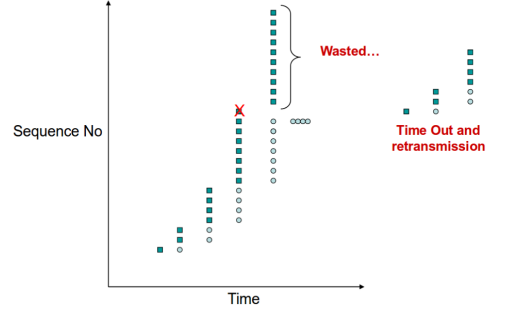
\includegraphics[scale=0.8]{tahoe}
  \caption[TCP Tahoe]{TCP Tahoe uses only timeouts to detect losses}
\end{figure}

\subsection{TCP Reno}
Characteristics:
\begin{itemize}
  \item Fast Retransmit/Fast Recovery (3 dupAcks to recover one packet loss)
  \item TCP Reno can recover from one packet loss without having a time out
\end{itemize}

\begin{figure}[h]
  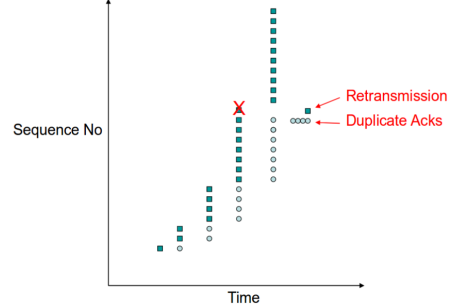
\includegraphics[scale=0.8]{fast_retransmit}
  \caption[TCP Reno 1]{TCP Reno - Fast Retransmission}
\end{figure}

\begin{figure}[h]
  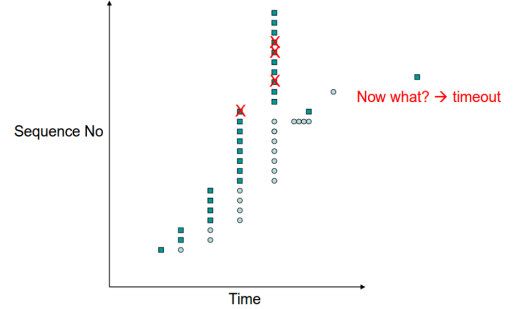
\includegraphics[scale=0.8]{reno}
  \caption[TCP Reno 2]{TCP Reno - more than one packet loss}
\end{figure}

\subsubsection{TCP New Reno}
TCP New Reno introduces partial ACKs to recover more packets without the use of
timeouts.
\begin{figure}[h]
  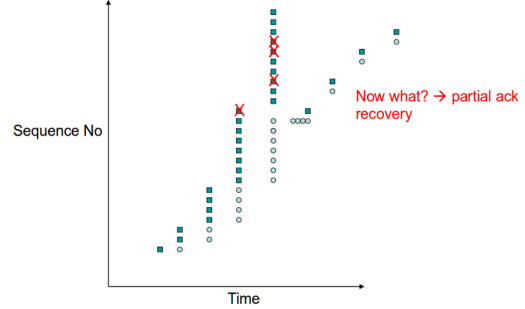
\includegraphics[scale=0.8]{partial_acks}
  \caption[TCP New Reno]{TCP New Reno - partial ACKs}
\end{figure}

\subsection{TCP SACK}
SACK means \textit{Selective acknowledgment}.

Returning ACKs declares which packets (even non contiguous) were received.
All non-received packets can be retransmitted and so it recovers from multiple
losses in just one RTT.
\begin{figure}[h]
  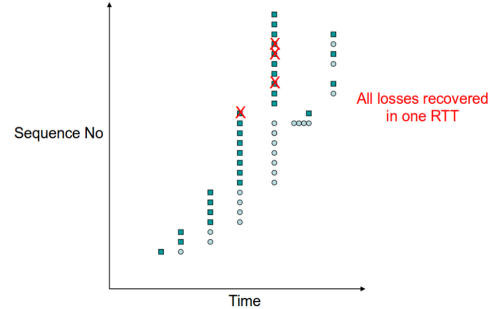
\includegraphics[scale=0.8]{sack}
  \caption[TCP SACK]{TCP SACK - Recovery from multiple losses in just one RTT}
\end{figure}
